\documentclass[]{article}
\usepackage{tikz,pgfplots}
\DeclareGraphicsRule{.tif}{png}{.png}{`convert #1 `dirname #1`/`basename #1 .tif`.png}

%opening
\title{CS 2024 Final Project: A Programmable Calculator with Cython and tkinter}
\author{Alex Xu (ax35), Brendan Taylor (bkt28), Chenxi Wu (cw538)\\ Erik Chan (ejc233), Elijah Wilt (ew356)}

\begin{document}

\maketitle

\section{Introduction}

For the final project of CS2024 we built a simple programmable calculator with C++/Python integration through Cython. It has the following features:
\begin{itemize}
	\item Infix arithmetic and relationship operators like $+$, $-$, $*$, $/$, $<$, $>$, $\%$.
	\item Mathematical functions like $\sin$, $\cos$, $\tan$, $\arcsin$, $\arccos$, $\arctan$, $\exp$, $\log$.
	\item Storing and retrieving values from variables labeled by numbers.
	\item A control structure that can be used to implement ``if'', ``while'' and ``do while'' statements.
	\item GUI written in Python with tkinter.
\end{itemize}

\section{Files and usage}

The following files are contained in the submitted .zip archive:
\begin{itemize}
	\item Makefile
	\item setup.py\\
	Python script for compiling with Cython.
	\item CALC.pyx\\
	The description of the interface between C++ and Python from the Python side.
	\item cal.h\\
	The description of the interface from the C++ side.
	\item cal.cpp\\
	The implementation of the calculator in C++.
	\item gui.py\\
	A GUI written with Python using tkinter.
	\item language\_spec.txt\\
	Specification of the programming language implemented by our calculator.
	\item testcases.txt\\
	Test cases we used in debugging. Besides basic arithmetics, it includes expressions that calculate factorial, Fibonacci numbers, finds roots with Newton's method, does bubble sort and count primes with the Sieve of Eratosthenes. 
\end{itemize}

To compile on a Linux or OSX machine, just type ``make''. To run, type ``python gui.py''. Enter the expression one want to evaluate on the large Edit box, then click the button labeled ``Evaluate''. Below is a screen shot.\\

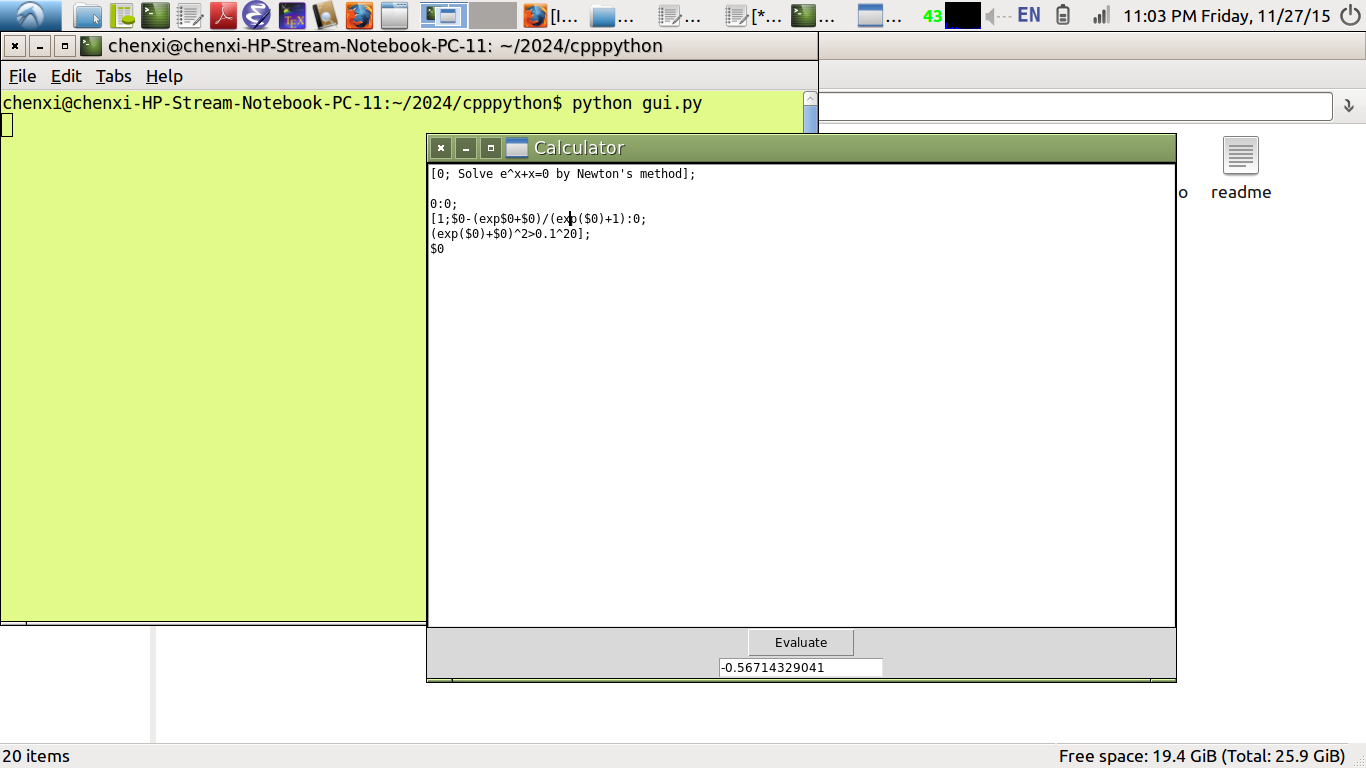
\includegraphics[scale=0.25]{screenshot.png}

\section{Implementation Details}
\subsection{The calculator}
We implemented 10 infix operators and 10 unary, prefix operators, as well as the bracket () and a control structure [], all defined and described in language\_spec.txt. The binary operators are implemented by a simple precedence climbing algorithm which is a modified version of recursive descent. Variables are implemented as an unordered\_map from the C++ standard library.

\subsection{The interface with Python}
On the C++ side, we made a class calc\_exp which has as its members an expression as a C++ string, the result of its evaluation, a boolean flag, the setters and getters of the expression, and a function eval(). After a change of the expression, when eval() is called for the first time, the expression is evaluated and the result is stored and returned. Further calls of eval() will return the stored result unless a change in expression reset the boolean flag.\\

On the Python side, we made a class CALC, with getters and setters of the expression and a evalexp() function all implemented by calling the corresponding functions in C++.

\subsection{GUI}
The GUI is written in Python with tkinter package and is rather simple and straightforward.


\end{document}
